% IMPORTANT: add or remove (comment out) the boolean '\solutiontrue' below to
% create the solution document or the exercise document respectively.
% First we create the switch to make either the exercises or the solutions
\newif\ifsolution\solutionfalse
% To create the solution uncomment '\solutiontrue'
\solutiontrue

\documentclass[a4paper,11pt]{article}

\title{System Security,
\ifsolution Solution \else \fi
Lab Report}

\author{George Cojocar, Andrin Jenal, Jonas Passerini}

\usepackage[T1]{fontenc}
\usepackage{ae, aecompl}
\usepackage{a4wide}
\usepackage{boxedminipage}
\usepackage{caption}
\usepackage{subcaption}
\usepackage{url}
\usepackage{graphicx}
\usepackage{enumerate}

% Some useful commands and environments
\usepackage{framed}
\newenvironment{solution}%
{\par{\noindent\small\textit{Solution:}}\vspace{-12pt}\begin{framed}}%
{\end{framed}\par}

\begin{document}
\maketitle

\section{General Hints for the reports}

To help you structuring the report on the labs, we provide you with some
questions to answer in the report and some \textbf{hints} you might need to
consider. Please, note that it is not an exhaustive list of questions.
Therefore, we advise you to include more information from your hacking
experience in the report.

\section{Lab Session: Side-channel attack}
In the lab session, the goal is to find the secret key used in a RSA
operation by analyzing the power consumption.
\begin{enumerate}[(a)]
\item Explain the setup to measure the power consumption of the sensor node
\ifsolution\begin{solution}
The setup used for power analysis attack consists of a single-board micro-controller, an AC/DC power supply and an oscilloscope (see Figure~\ref{fig:setup}). The micro-controller is powered by the external power supply, and it performs an encryption and a decryption sequence when it is turned on. The power consumption during cryptographic operations is measured by the oscilloscope which is connected to the micro-controller's power pins.

\makeatletter
\begin{center}
\def\@captype{figure}

\begin{subfigure}[b]{0.7\textwidth}
	\includegraphics[width=\textwidth]{screenshots/20151008_150146_sharp.jpg}
\end{subfigure}
\caption{Shows the initial setup with the micro-controller and the oscilloscope.}
\label{fig:setup}

\end{center}
\makeatother

\end{solution}\fi

\newpage
\item What technique did you use to improve the measurement noise in
the power trace?
\ifsolution\begin{solution}

\makeatletter
\begin{center}
\def\@captype{figure}

\begin{subfigure}[b]{0.47\textwidth}
	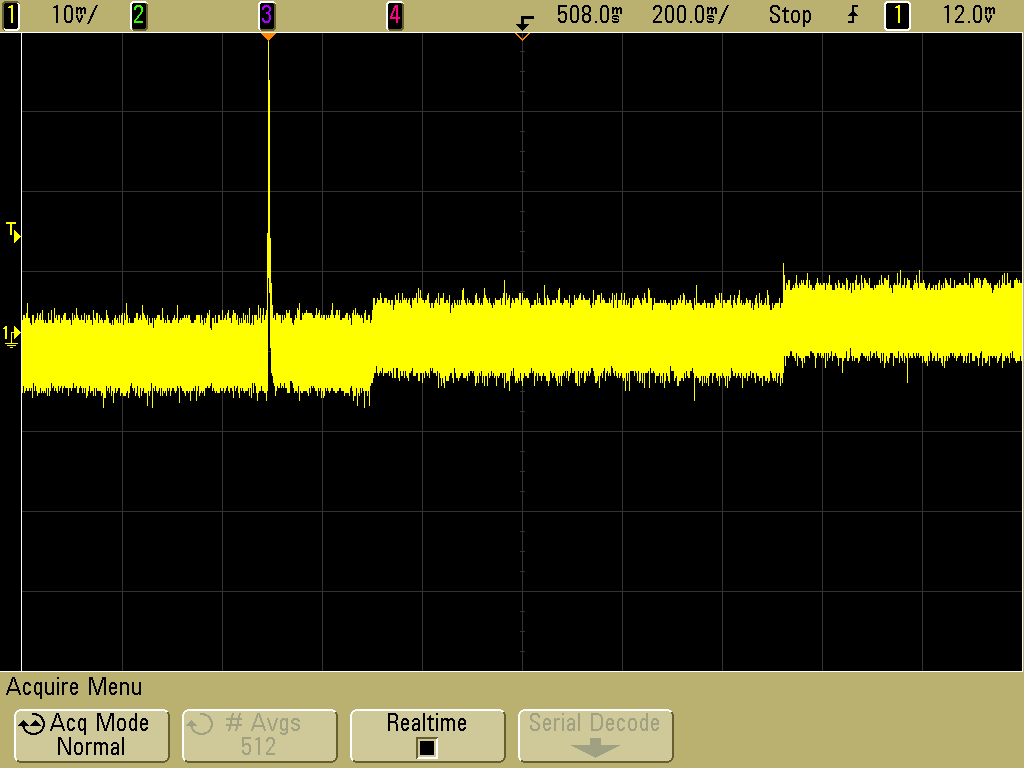
\includegraphics[width=\textwidth]{screenshots/print_000.png}
	\caption{Power measurement of a single signal using the oscilloscope.}
	\label{fig:single_signal}
\end{subfigure}
\begin{subfigure}[b]{0.47\textwidth}
	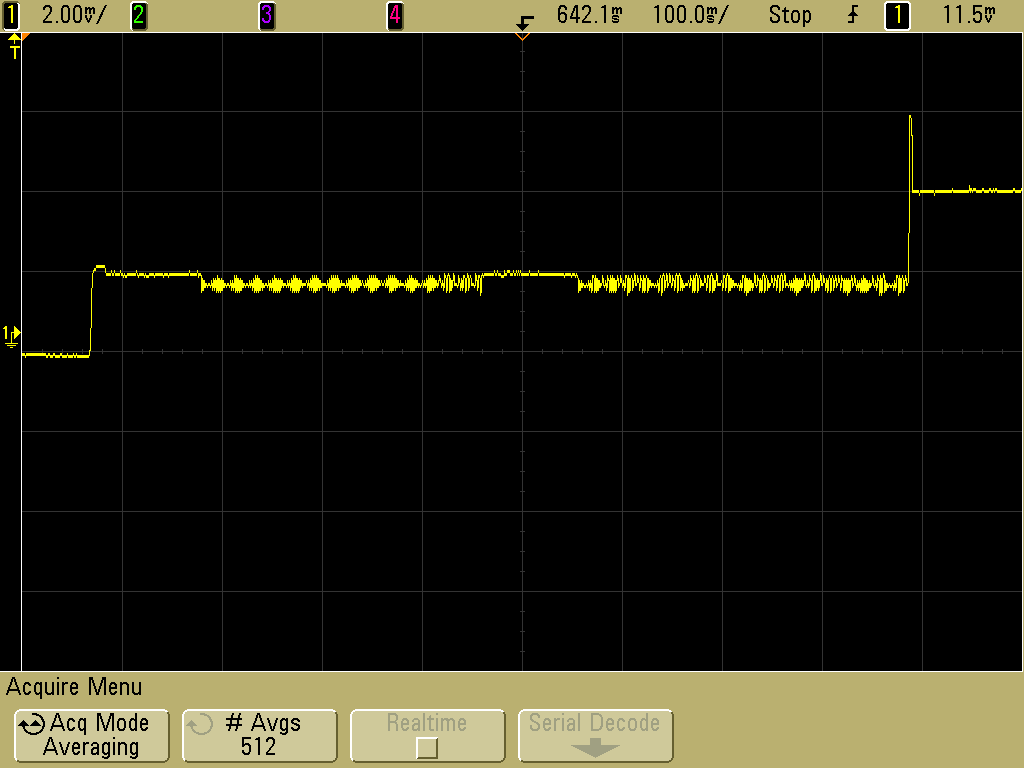
\includegraphics[width=\textwidth]{screenshots/print_002.png}
	\caption{Averaged power measurement of 512 signals using the oscilloscope.}
	\label{fig:averaged_signal}
\end{subfigure}

\caption{Effect of averaging on the measured signal compared to a single signal measurement.}
\label{fig:averaging}

\end{center}
\makeatother


The method used to reduce the noise on a measured signal was signal averaging. We set up a trigger and acquired the noisy signal 512 times. The oscilloscope added up all acquisitions and divided by 512. This technique significantly reduced the level of noise as one can see when comparing the power measurement of a single signal in Figure \ref{fig:single_signal} to the averaged power measurement in Figure \ref{fig:averaged_signal}.
\end{solution}\fi



\item To which horizontal resolution did you set the oscilloscope to read out
the bits? How did you find this value?
\ifsolution\begin{solution}
The value of horizontal resolution was 2 seconds. We found this value by configuring the maximum resolution available in order to achieve the most accurate period and frequency measurements. Afterwards we adjusted the horizontal scale until the whole signal was visible.
\end{solution}\fi

\newpage
\item What is the key that you could see? Explain how you are able to
see the key and what leads to differences in the power consumption.
Mark the different bits in a picture.
\ifsolution\begin{solution}

\par The RSA decryption is implemented by using the square and multiply exponentiation algorithm. Each of the two operations has a different power consumption pattern, that can be observed on an oscilloscope. For this reason, one can apply simple power analysis and extract the private key bit by bit as follows:

\begin{itemize}
  \item If the squaring is followed by a multiplication, this bit of the exponent is one
  \item If the squaring is followed by another squaring, this bit of the exponent is zero
\end{itemize}

A shorter operation consists only of squaring and therefore represents a zero while a longer operation both consists of squaring and multiplication and accordingly represents a one. This information can be used to directly read the key from the power measurement as one can clearly distinguish between shorter and longer operations.
Figure \ref{fig:key_extraction} shows the extraction of the public and private key based on the power measurements. In our experiment, the last 16 bits of the private key are 0x2A0B as shown in Figure \ref{fig:private_key} and the last 16 bits of the public key are 0x5ABB as shown in Figure \ref{fig:public_key}.

\makeatletter
\begin{center}
\def\@captype{figure}

\begin{subfigure}[b]{0.7\textwidth}
	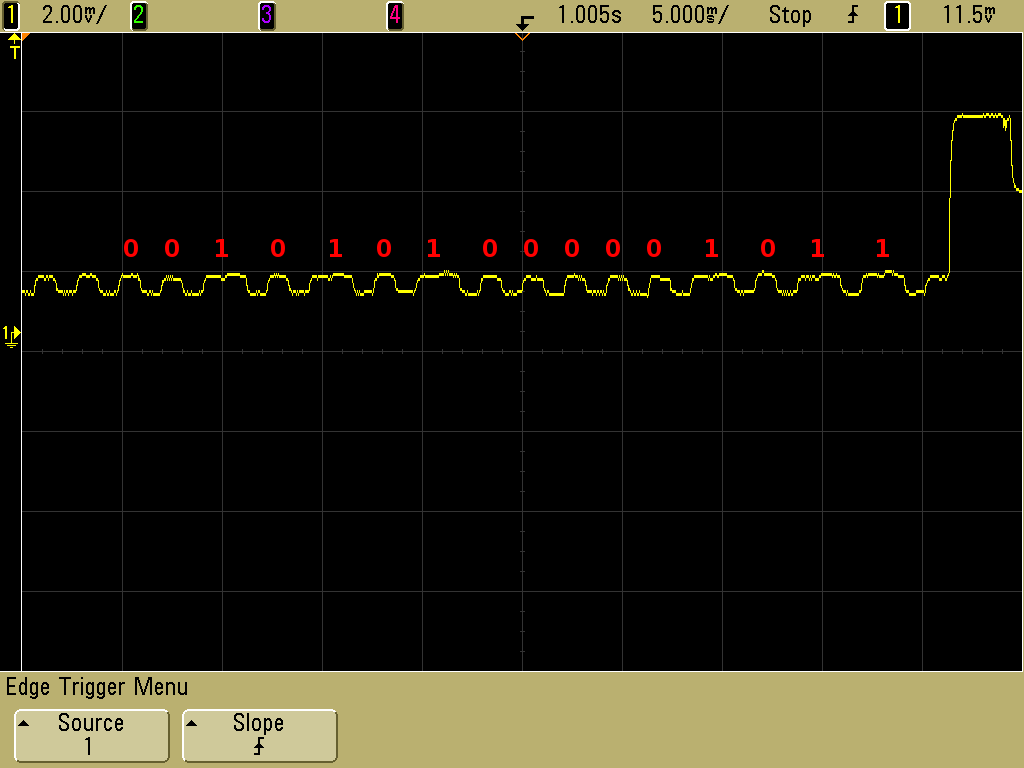
\includegraphics[width=\textwidth]{screenshots/print_006_bits.png}
	\caption{Extraction of the last 16 bits of the private key (0x2A0B).}
	\label{fig:private_key}
\end{subfigure}
\begin{subfigure}[b]{0.7\textwidth}
	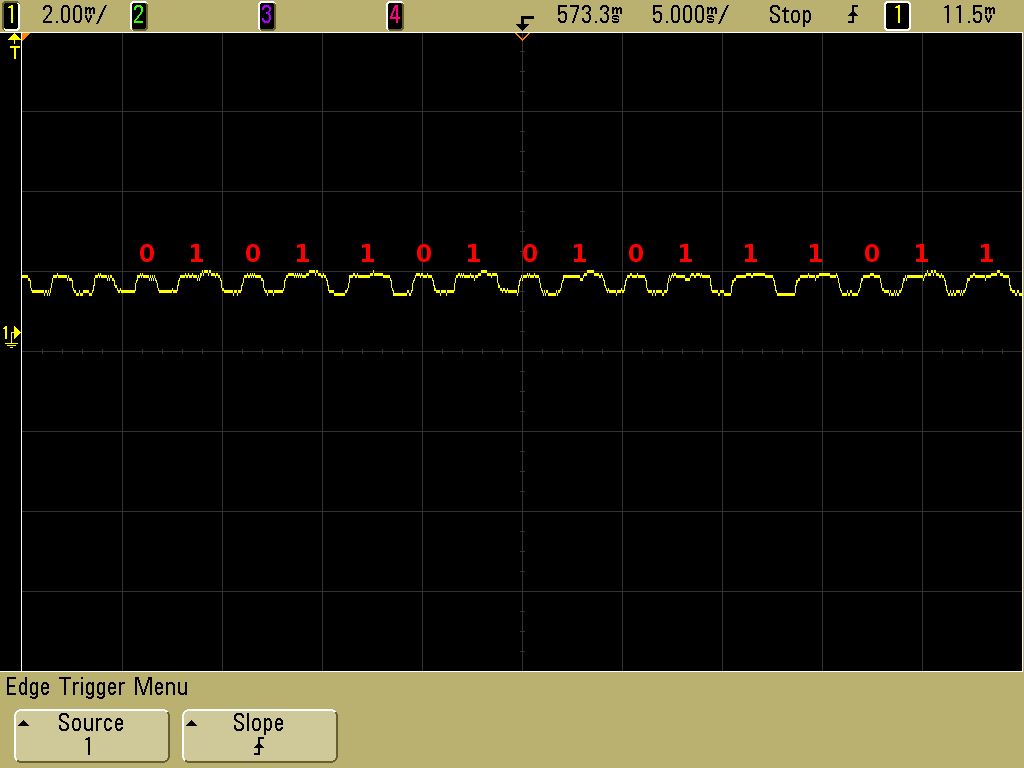
\includegraphics[width=\textwidth]{screenshots/print_003_bits.png}
	\caption{Extraction of the last 16 bits of the public key (0x5ABB).}
	\label{fig:public_key}
\end{subfigure}

\caption{Key extraction based on the averaged measurement while performing the encryption and decryption. Bit 1 is represented by a larger working cycle and bit 0 by a smaller one.}
\label{fig:key_extraction}

\end{center}
\makeatother



\end{solution}\fi

\end{enumerate}

\begin{thebibliography}{---}
\bibitem[1]{syssec}
        Srdjan Capkun, Adrian Perrig,
        \emph{System Security},
        ETH, AS 2015
\end{thebibliography}

\end{document}
